\documentclass{scrartcl}

\usepackage{amssymb}
\usepackage{amsmath}
\usepackage{listings}

\usepackage{graphicx} % Required for including pictures
\usepackage{float} % Allows putting an [H] in \begin{figure} to specify the exact location of the figure
\usepackage{wrapfig} % Allows in-line images such as the example fish picture


\begin{document}

\title{Phylodynamics:  How the Study of Evolution Benefits Society!}

\subtitle{(-while also just being really, ridiculously interesting)}
\author{Alex Popinga, Computational Evolution Group, UoA}
\date{}
\maketitle
%\subtitle{(-while also just being really, ridiculously interesting)}
%\author{Alex Popinga and Alexei Drummond}
%\date{\normalsize{Computational Evolution Group, UoA}}
%\maketitle

\section{Phylogenetics, A review of}

As Prof Alexei Drummond explained in his lecture on 9 March, \textbf{\textit{phylogenetics}} is the study of evolutionary relationships.  
These relationships can be both effectively and meaningfully represented by a tree, such as the one shown in Fig.1.
The concept and maths are the same for family trees, gene trees, species trees, etc.  

\begin{figure}[H] 
\center
{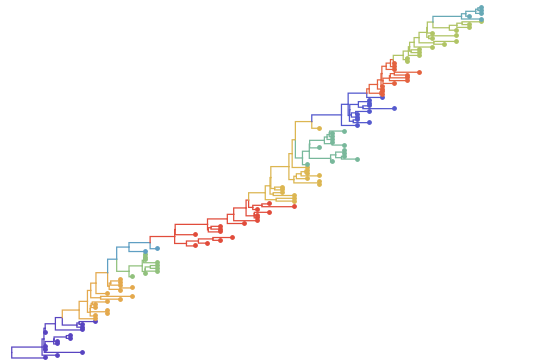
\includegraphics[width=0.7\linewidth]{tree.png}}
\caption{A tree showing the relationships between individual H3N2 virus sequences (represented by the tips, or leaves). Image credit: www.trevorbedford.com}
\label{sequences}
\end{figure}

\vspace{2mm}
\noindent{So why do we care?  Firstly, it's just inherently interesting; all this genetic diversity you see around you - from viruses to 
turkeys to ferns to your best friend's aunt's neighbor's second cousin twice removed - arose from millions of years of evolution, and we are all connected somehow!  
Also, as it turns out, such insight can be incredibly useful, too.}

%Of course, the larger the tree, the more unique ways 
%of drawing the tree - that is, the greater the number of possible unique ways to describe these relationships.  

\vspace{2mm}
\noindent{The study of \textbf{\textit{phylodynamics}} is a subset of phylogenetics that is concerned specifically with the evolutionary 
relationships of viruses that cause infectious diseases.  (It is a portmanteau of ``phylogenetics" and epidemiological ``dynamics".)  
Let's focus on the phylogenetics part first.  Suppose some medical people and other scientists already did the grueling lab work of taking samples of 
viruses from sick people and sequencing them.  What do we do now?}

\begin{itemize}
	\item *Step `0':  Align genetic sequences from the viruses we're interested in.
	\item \hspace{0.5mm} Step `1':  Infer a tree to give us insight into the relationships between said viruses.
\end{itemize}

\noindent{\footnotesize{*We're computer science nerds, so we're allowed to start numbering at `0'.}}

%\begin{equation}
%\end{equation}

\subsection{Aligning sequences}

A sequence alignment shows us regions of similarity and dissimilarity between a list of sequences (and can then be used for inferring trees).
Some sequences, such as those shown in Fig.2, have a ``best" alignment that is obvious to the eye and can easily be done by hand.

\begin{figure}[H] 
\center
{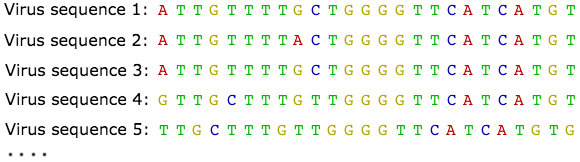
\includegraphics[width=0.7\linewidth]{FluSequence0.png}}
\caption{A list of unaligned nucleotide sequences.}
\label{sequences}
\end{figure}

\vspace{2mm}
\noindent{However, in real analyses the sequences are much longer than shown in Fig.2 - (in fact, they must be, otherwise there is not enough 
information to tell us anything with enough certainty to be useful!) - and also a best alignment may not be all that obvious.}

\vspace{2mm}
\textbf{How do we go about lining up these sequences?}  There are several different ways to align sequences, even programmatically (and trust me, you'll 
want to align them programmatically).  For now, let's focus on getting started.  

\begin{itemize}
\item \textbf{GOAL:}  Write a program to solve our problem - that is, to align sequences.
\item \textbf{Step 0:}  Count the number of `As', `Ts', `Cs', and `Gs' in each sequence. 

\texttt{http://rosalind.info/problems/dna/}
\item \textbf{Step 1:}  Find a pattern, or motif, between the sequences. 

\texttt{http://rosalind.info/problems/subs/}
\end{itemize}


\subsection{Building a tree}

Now that we have our sequence alignment, we can think about how these sequences relate to each other.  If each sequence represents the tip of a tree,

\vspace{2mm}
[Give them a sequence alignment to load into BEAUti... run BEAST analysis]

\section{The Dynamics of Epidemics}

\subsection{The SIR model}

A population that has not been introduced to a particular infectious agent is called a \textit{na\"\i ve} population.  The people in the population who are 
\textit{susceptible} to infection once the contagion is introduced can be classed together into a subpopulation we'll call ``S".  Once they become 
infected (and are now infectious), they go into another subpopulation class we'll call ``I".  If the type of infection in question then has 
another stage that effectively removes people from both susceptible and infected classes - such as recovery with immunity, quarantine, or death - 
then we also have a removed class ``R".  We call a model with S, I, and R classes an \textit{SIR model}, because we're succinct like that. 

\vspace{3mm}
\textbf{What is the purpose of describing models like SIR?}  Well, we can estimate important parameters from these models, such as transmission rates and rates of removal 
(respectively, $\beta$ and $\gamma$ in Fig.3), which allow us to quantify how rapidly an epidemic outbreak is spreading, etc.

\begin{figure}[H] 
\center
\quad
{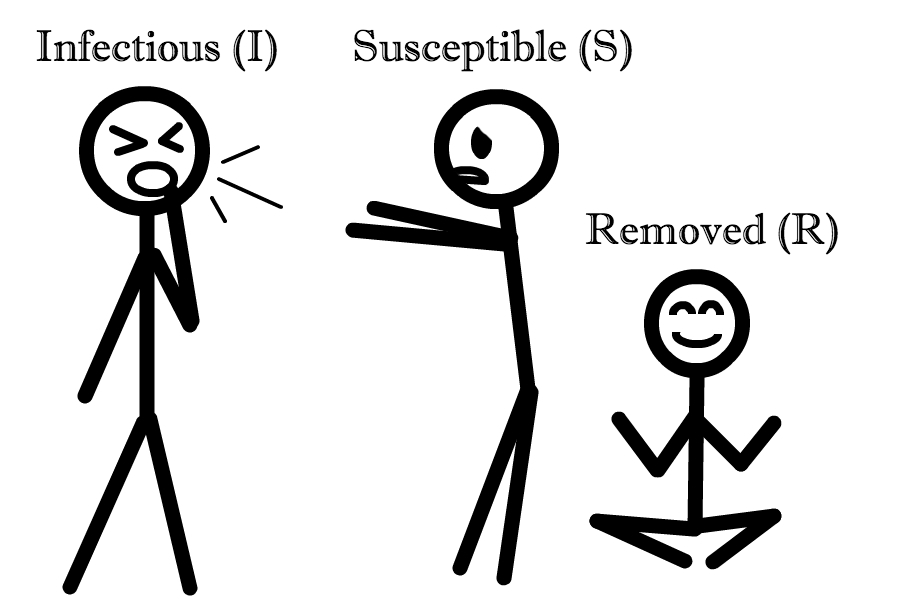
\includegraphics[width=0.4\linewidth]{SIR.jpg}}
\quad
{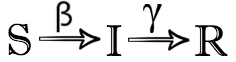
\includegraphics[width=0.25\linewidth]{SIRgraphic.jpg}}
\caption{A simple, closed SIR model with a rate of infection $\beta$ from the susceptible S to infected I class and a rate of removal $\gamma$ from infected I to removed R class.}
\label{sequences}
\end{figure}

[Give them MASTER XML for SIR simulation, have them fiddle with the parameters and population sizes, observe effects by loading JSON in R]

\section{Phylodynamics}

\subsection{Sequences to SIR model}

\subsection{Phylodynamics in BEAST 2}

[Give them Coalescent SIR and/or BDSIR XML... look at log file in Tracer, tree file in IcyTree or FigTree]

%----------------------------------------------------------------------------------------
%	BIBLIOGRAPHY
%----------------------------------------------------------------------------------------
\newpage
\begin{thebibliography}{99} % Bibliography - this is intentionally simple in this template

%\bibitem[{{Vaughan and Drummond\/}, 2013}]{MASTER}
%{\sc Vaughan, T.~G.} and {\sc A.~J. Drummond}, 2013.
%A Stochastic Simulator of Birth–Death Master Equations with Application to Phylodynamics.
%\newblock Mol. Biol. Evol.
 
\end{thebibliography}

%----------------------------------------------------------------------------------------
\end{document}